\documentclass[11pt,a4paper]{article}
\usepackage[T5]{fontenc}
\usepackage[utf8]{inputenc}
\usepackage[vietnamese]{babel}
\usepackage{tgtermes}
\usepackage[margin=2.3cm]{geometry}
\usepackage{booktabs,graphicx,xcolor,array}
\usepackage[hidelinks]{hyperref}
\usepackage{caption}
\captionsetup{font=small,labelfont=bf}
\usepackage{titlesec}
\titleformat{\section}{\large\bfseries}{\thesection.}{0.6em}{}
\titleformat{\subsection}{\normalsize\bfseries}{\thesubsection.}{0.6em}{}
\setlength{\parskip}{0.35em}
\setlength{\parindent}{0pt}
\newcommand{\up}[1]{\textcolor{teal!70!black}{\textbf{#1}}}
\newcommand{\down}[1]{\textcolor{red!65!black}{#1}}

\title{\vspace{-1.2cm}\textbf{Báo cáo tiến độ Phase 3}\\[0.25em]
\large Ứng dụng AI trong gán nhãn ảnh y tế cho bệnh đau thắt lưng}
\author{Trung Kiên \quad\textbar\quad GVHD: Phan Trọng Nhân}
\date{09/09/2026}

\begin{document}
\maketitle
\vspace{-0.9cm}

\section{Tóm tắt}

Báo cáo tổng hợp kết quả Phase 3, đối chiếu với mốc đã trình bày trước hội đồng ở Phase 2.
Ba nhóm việc đã hoàn thành: (i) hoàn thiện phần mềm gán nhãn có vòng phản hồi bác sĩ;
(ii) bốn thực nghiệm GPU tìm hướng cải thiện lớp Severe; (iii) chẩn đoán nguyên nhân
điểm yếu ở nhãn lỗ liên hợp và một khung đánh giá khả diễn giải có kiểm chứng.

Kết quả đáng kể nhất là \textbf{chẩn đoán được nguyên nhân} khiến nhãn lỗ liên hợp
(\textit{neural foraminal narrowing}) luôn kém: quy trình cắt ảnh cũ lấy vùng ảnh từ chuỗi
Sagittal T2 trong khi bác sĩ chấm nhãn này trên Sagittal T1, và đo trong không gian bệnh nhân
cho thấy \textbf{32{,}2\% (trái) và 47{,}2\% (phải)} vùng cần chấm nằm ngoài độ sâu ảnh
mà mô hình được cho. Sau khi cắt riêng theo từng bên trên T1, AUPRC lỗ liên hợp
tăng \up{+0{,}054} và \up{+0{,}039} so với Phase 2.

Báo cáo cũng ghi lại bốn kết quả âm và hai lỗi phương pháp đã phát hiện, vì chúng ảnh hưởng
tới cách diễn giải số liệu cũ.

\section{Phần mềm gán nhãn}

Ứng dụng web (FastAPI + React/Cornerstone3D) cho phép tải ảnh MRI, xem theo lát, chạy mô hình
chấm 11 nhãn bất thường, và \textbf{ghi nhận chỉnh sửa của bác sĩ như phản hồi chuyên gia}.
Quy mô hiện tại: 16.426 dòng Python, 2.452 dòng frontend, 24 tệp kiểm thử.

\begin{figure}[htbp]
\centering
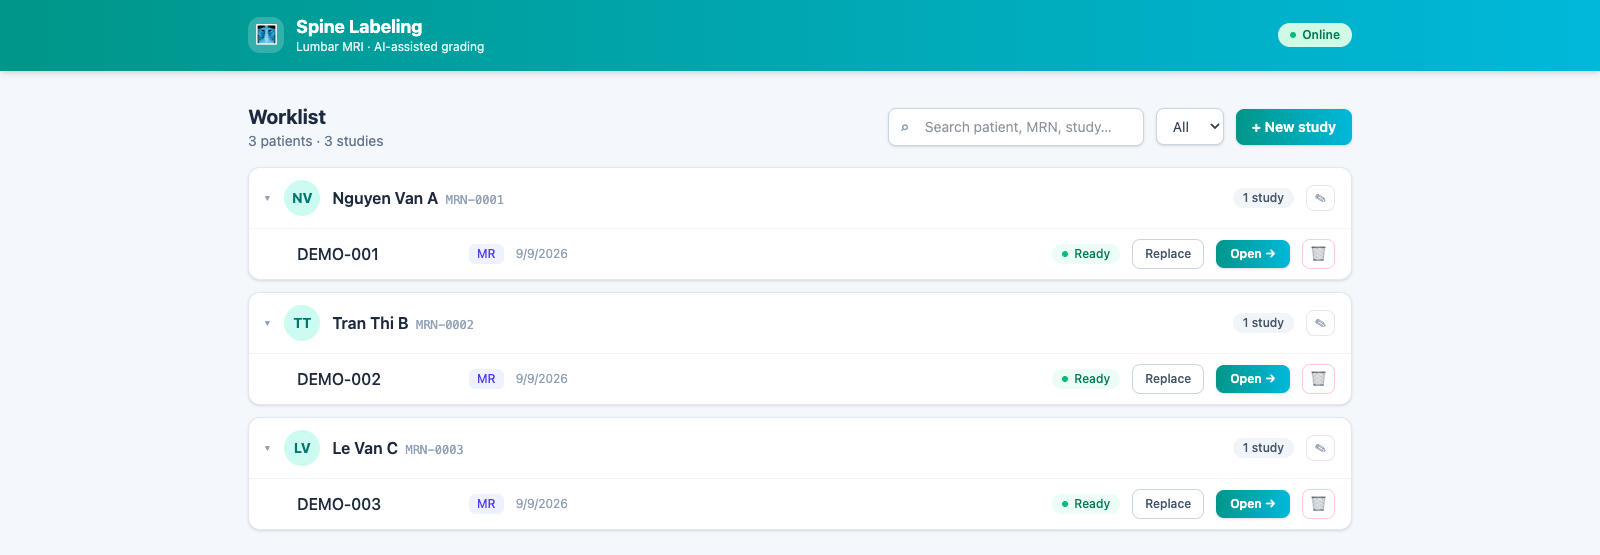
\includegraphics[width=0.92\textwidth]{figures/app_worklist.png}
\caption{Màn hình danh sách ca. Mỗi bệnh nhân có thể chứa nhiều lần chụp; trạng thái
\textit{Ready} nghĩa là ảnh đã tải xong và sẵn sàng chấm.}
\label{fig:worklist}
\end{figure}

\begin{figure}[htbp]
\centering
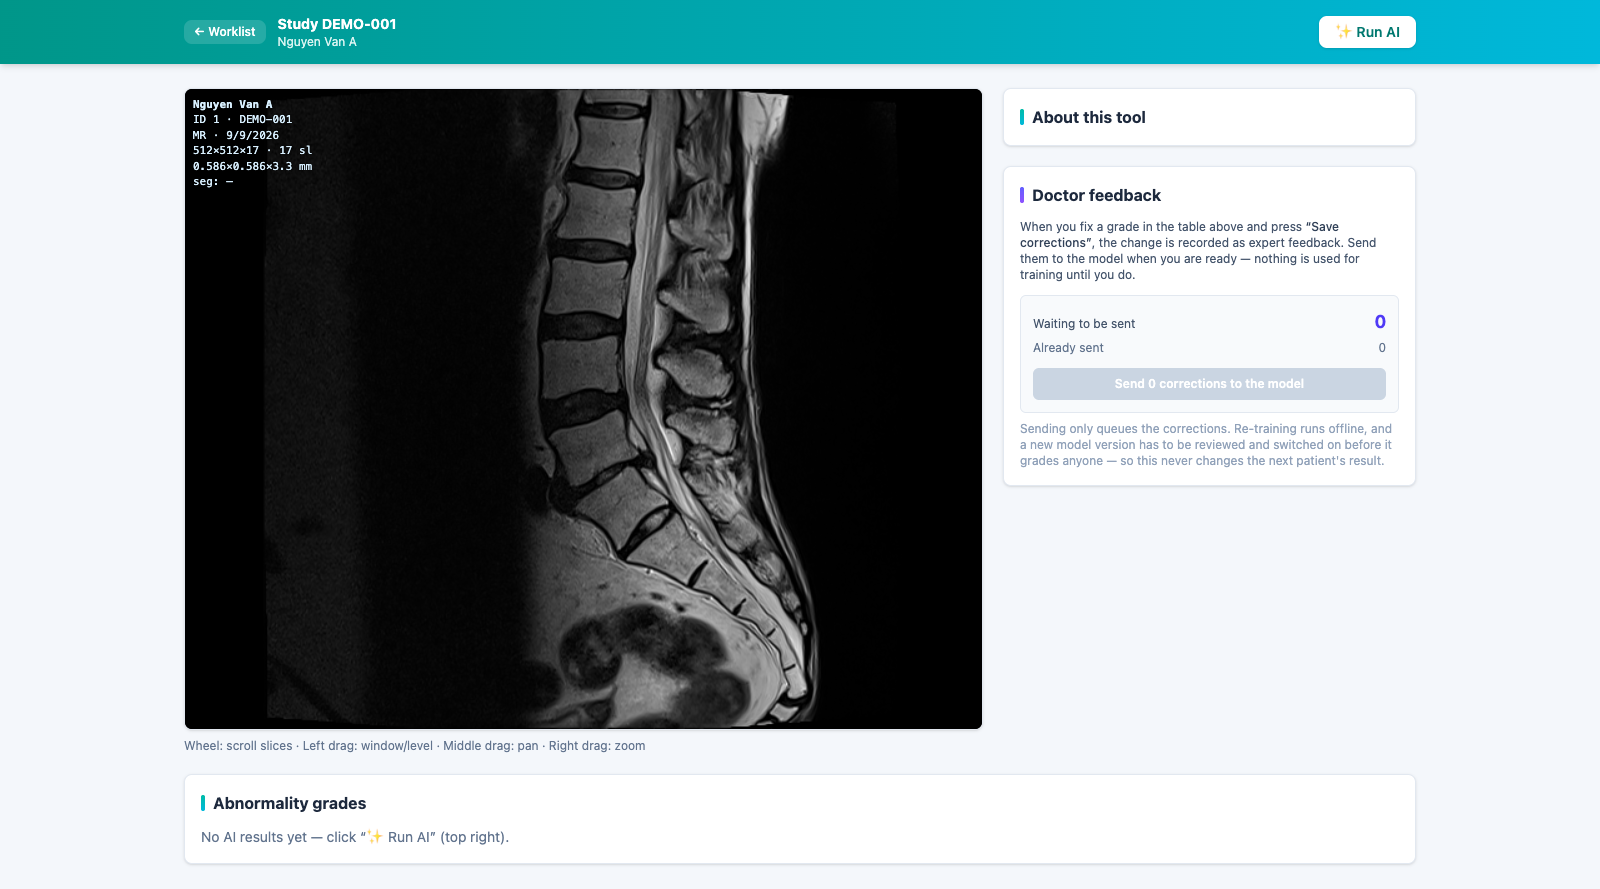
\includegraphics[width=0.92\textwidth]{figures/app_viewer.png}
\caption{Màn hình đọc ảnh, hiển thị chuỗi Sagittal T2 (512$\times$512$\times$17,
0{,}586$\times$0{,}586$\times$3{,}3 mm). Bảng \textit{Abnormality grades} nằm dưới ảnh cho phép
bác sĩ sửa từng nhãn; khối \textit{Doctor feedback} bên phải gom các chỉnh sửa thành hàng đợi
huấn luyện.}
\label{fig:viewer}
\end{figure}

Điểm thiết kế đáng lưu ý ở Hình~\ref{fig:viewer}: chỉnh sửa của bác sĩ \textbf{không tác động
ngay} tới mô hình. Chúng được xếp hàng, việc huấn luyện lại chạy ngoại tuyến, và phiên bản mô hình
mới phải được duyệt rồi mới kích hoạt. Điều này tránh tình huống kết quả của bệnh nhân sau bị
thay đổi bởi chỉnh sửa của bệnh nhân trước.

\section{Vòng phản hồi bác sĩ: phương pháp}

Mục~2 mô tả vòng phản hồi ở mức thao tác. Mục này nói phần phương pháp: cơ chế cập nhật là gì,
gọi tên thế nào trong tài liệu, đo bằng gì, và hiện đã làm tới đâu.

\subsection{Gọi tên cho đúng}

Hệ thống là \textbf{human-in-the-loop continual learning} dạng \textbf{batch/ngoại tuyến},
kịch bản \textbf{new-instance (NI)} --- cùng bài toán chấm điểm, cùng không gian nhãn, chỉ thêm
mẫu mới đã được bác sĩ hiệu chỉnh --- cập nhật bằng \textbf{rehearsal (replay)} và có
\textbf{cổng phê duyệt của người}.

Bóc từng vế: kịch bản NI theo bộ ba NI/NC/NIC của Lomonaco và Maltoni (CORe50, CoRL 2017), vì
không thêm lớp mới và không thêm tác vụ mới; nhãn cố định \textit{Normal/Mild--Moderate--Severe}
nên không phải class-incremental theo phân loại của van de Ven và Tolias (arXiv:1904.07734);
vai trò kép của bác sĩ --- vừa sinh nhãn vừa gác cổng --- là định nghĩa human-in-the-loop trong
khảo sát của Budd, Robinson và Kainz (\textit{Medical Image Analysis}, 2021).

Ba cách gọi cần tránh, vì đều sai và đều làm yếu lập luận. Thứ nhất, \textbf{không} gọi là
\textit{online learning}: online là cập nhật ngay theo từng ca, còn ở đây cố ý gom lô và chạy
ngoài giờ --- chính cái ``cố ý không'' đó mới là đóng góp. Thứ hai, \textbf{không} gọi trần là
\textit{fine-tuning}: fine-tune trần trên vài chục ca là \textit{iterative fine-tuning}, chưa phải
continual learning, vì thiếu cơ chế chống quên; thứ nâng nó lên là ba chốt ở mục~3.2. Thứ ba,
\textbf{không} nhận là \textit{active learning}: active learning là mô hình tự chọn ca nó không
chắc để hỏi, còn ở đây bác sĩ tự chọn ca. Đây là phần duy nhất trong phân loại còn thiếu, và nó
rẻ vì đầu ra đã có xác suất; xếp vào hướng phát triển.

\subsection{Cơ chế cập nhật và ba chốt an toàn}

Mô hình gồm hai phần: phần nền ResNet34-3D kèm CBAM (khoảng 63 triệu tham số, ``học cách nhìn'')
và ba đầu phân loại (khoảng 50 nghìn tham số, ``học cách phán''). Với vài chục ca chỉnh sửa,
huấn luyện 63 triệu tham số sẽ học thuộc đúng mấy ca đó và quên gần mười nghìn ca RSNA.

Vì vậy cách cập nhật là \textbf{chỉ huấn luyện ba đầu, đóng băng phần nền}. Giả định nền là bác sĩ
sửa nhãn phần lớn vì \textit{ngưỡng phán} lệch chứ không phải vì mô hình \textit{nhìn} sai; tỉ lệ
50 nghìn tham số trên vài chục mẫu cũng là tỉ lệ chấp nhận được. Kèm theo là ba chốt, mỗi chốt
chặn một kiểu hỏng không phát ra lỗi:

\begin{enumerate}
\itemsep0.15em
\item \textbf{Đóng băng BatchNorm.} Đóng băng phần nền chỉ tắt gradient, trong khi BatchNorm cập
nhật thống kê \textit{không} qua gradient. Một lô bốn mẫu sẽ đè thống kê tích luỹ từ toàn bộ tập
huấn luyện. Đây là nguyên nhân đã được ghi nhận của việc quên thảm khốc khi thích nghi mô hình y tế
trên tập nhỏ (arXiv:2011.08096).
\item \textbf{Bộ đệm replay.} Trộn khoảng 200 đĩa đệm gốc vào mỗi lượt cập nhật. Không có nó, mô
hình chỉ thấy những ca bị sửa và tưởng dữ liệu thật đều như vậy.
\item \textbf{Cổng macro-F1.} Chỉ giữ trọng số mới nếu macro-F1 tăng trên tập đánh giá đã đóng băng.
\end{enumerate}

Hình~\ref{fig:feedback_loop} vẽ toàn bộ vòng lặp theo bốn dải: trực tuyến (ứng dụng phục vụ), thu
thập (tách ``lưu'' khỏi ``gửi''), ngoại tuyến (huấn luyện lại theo lô và kiểm chứng), và triển khai
(người duyệt, có thể hoàn tác). Nét liền là thành phần đã cài đặt và đã kiểm thử; nét đứt là dự
kiến --- hiện chỉ có hai hộp nét đứt, là \textit{active learning} và \textit{kiểm tra chất lượng
nhãn}.

\begin{figure}[htbp]
\centering

\includegraphics[width=\textwidth]{figures/feedback_loop_tikz.pdf}
\caption{Vòng lặp phản hồi bác sĩ theo cơ chế human-in-the-loop continual learning dạng batch.
Nét liền: thành phần đã cài đặt và kiểm thử; nét đứt: dự kiến.}
\label{fig:feedback_loop}
\end{figure}

Bảng~\ref{tab:vi_sao_khong} giải thích vì sao không chọn các hướng cập nhật khác. Lý do chung là ở
vùng vài chục mẫu, replay có bằng chứng y tế mạnh nhất, còn các hướng còn lại hoặc cần nhiều mẫu
hơn, hoặc cần thành phần mà ứng dụng hiện không chạy.

\begin{table}[htbp]
\centering
\caption{Vì sao chọn head-only kèm replay thay cho các hướng cập nhật khác.}
\label{tab:vi_sao_khong}
\small
\begin{tabular}{@{}lp{9.2cm}@{}}
\toprule
\textbf{Hướng} & \textbf{Lý do không chọn} \\
\midrule
Head-only + replay + BN đóng băng & Đang dùng. Rẻ, bằng chứng y tế mạnh nhất ở vùng dữ liệu ít \\
EWC & Ma trận Fisher cần dữ liệu cũ; ở vài chục mẫu ước lượng không đáng tin. Thực nghiệm trên ảnh da liễu cho thấy replay thắng EWC ở mọi cấu hình \\
LwF & Bằng chứng y tế mỏng, không mạnh hơn replay \\
LoRA / adapter & Cần từ 50 mẫu trở lên; thêm phụ thuộc, thừa ở quy mô này \\
Tip-Adapter / prototype & Không thể quên và hoàn tác tức thì, nhưng cần BiomedCLIP, trong khi ứng dụng đang chạy nhánh CBAM \\
Huấn luyện lại toàn bộ & Quên thảm khốc khi số mẫu nhỏ \\
\bottomrule
\end{tabular}
\end{table}

\subsection{Chuẩn bị dữ liệu từ chỉnh sửa}

Chỉnh sửa của bác sĩ không được dùng trực tiếp. Bước dựng dữ liệu làm bốn việc. Một, khử trùng lặp:
mỗi cặp (ca, ô nhãn) chỉ lấy lần sửa \textit{mới nhất}, vì bác sĩ có thể sửa đi sửa lại một ô. Hai,
chỉ lấy các lô đã gửi, và lấy được theo đúng một mã lô, để một lượt huấn luyện cũ tái lập được
chính xác những gì nó từng thấy. Ba, \textbf{cắt lại vùng ảnh} từ ảnh gốc và mặt nạ phân vùng bằng
đúng hàm mà lúc chấm đã dùng, cho ra khối $(9, 112, 224)$ --- không lưu ảnh tại thời điểm sửa, để
tránh lệch giữa lúc huấn luyện và lúc phục vụ. Bốn, ô nào bác sĩ không đụng tới thì gán $-1$, khớp
quy ước \textit{ignore\_index} mà nhánh huấn luyện chính đang dùng, nghĩa là không bịa nhãn cho
những đầu ra bác sĩ không nhận xét.

Ngoài dữ liệu chỉnh sửa, một lượt cập nhật còn cần hai tập nữa: tập replay khoảng 200 đĩa đệm gốc,
và tập đánh giá đã đóng băng. Cả hai lấy từ bộ RSNA 2024 đã tiền xử lý.

\subsection{Giao thức đánh giá và cổng chặn}

Tập đánh giá được \textbf{chốt trước khi thu thập bất kỳ chỉnh sửa nào}: 200 dòng, đóng băng ngày
26/07/2026, kèm tệp kê khai ghi SHA-256 của các dòng đã chọn cùng hạt giống và thời điểm, và có
lệnh kiểm tra lại để chứng minh tập không đổi. Điều này bắt buộc chứ không phải cho chặt chẽ: nếu
chọn tập đánh giá \textit{sau} khi đã biết bác sĩ sửa những đĩa nào, con số đo được phản ánh cách
chọn chứ không phản ánh mô hình, và không có cách nào dựng lại bảo đảm đó về sau.

Chỉ tiêu quyết định là \textbf{macro-F1}, không phải độ chính xác. Lớp \textit{Severe} hiếm, nên một
mô hình sập về đoán \textit{Normal/Mild} cho mọi ô vẫn đạt độ chính xác trung bình cao trong khi mất
hết giá trị lâm sàng --- đúng lớp mà đề tài sinh ra để cải thiện. Trọng số mới chỉ được ghi ra tệp
khi macro-F1 sau lớn hơn trước; không đạt thì bỏ, và tệp trọng số giữ lại có nhúng sẵn số đo
trước/sau để người duyệt nhìn số mà quyết.

\subsection{Vì sao ``theo lô, ngoại tuyến, có người duyệt'' là thiết kế đúng}

Hướng dẫn của FDA tháng 12/2024 về \textit{Predetermined Change Control Plan} (PCCP) cho phần mềm
y tế dùng trí tuệ nhân tạo cho phép nhà sản xuất khai báo trước phạm vi thay đổi --- tần suất, giới
hạn dữ liệu, quy trình kiểm chứng, cách hoàn tác --- và sau đó cập nhật trong phạm vi đó mà không
phải xin duyệt lại từ đầu. Điểm mấu chốt là hướng dẫn này áp cho \textbf{cập nhật theo lô, ngoại
tuyến}, không áp cho học trực tuyến liên tục. Đạo luật AI của Liên minh châu Âu, hiệu lực
01/08/2024, cùng quy định về thiết bị y tế cũng đòi có giám sát của người và hậu kiểm.

Nghĩa là thiết kế ``gom lô, chạy ngoài giờ, người bấm duyệt, hoàn tác được'' không phải làm cho
đơn giản mà là làm cho đúng khung quản lý. Đây là lập luận nên nói thẳng khi bảo vệ, vì nó biến một
điểm trông như hạn chế thành một lựa chọn có căn cứ.

\subsection{Chỉnh sửa của bác sĩ không phải chân lý}

Một nghiên cứu ba người đọc trên ảnh MRI thắt lưng thoái hoá cho thấy chỉ số đồng thuận Cohen's
$\kappa$ với thang Pfirrmann chỉ đạt 0{,}68, tức hai bác sĩ bất đồng khoảng một phần ba số ca.
Do đó việc một bác sĩ sửa nhãn của mô hình không đương nhiên có nghĩa mô hình sai, và nuốt toàn bộ
chỉnh sửa vào tập huấn luyện có nguy cơ dạy mô hình thiên theo cách đọc của một người.

Hướng xử lý theo \textit{confident learning} (Northcutt, Jiang và Chuang, JAIR 2021) là đánh dấu
những chỉnh sửa mâu thuẫn với dự đoán mà mô hình đang rất tự tin để xem lại, thay vì đưa thẳng vào
huấn luyện. Lý tưởng là mỗi ca có ít nhất hai bác sĩ đọc độc lập; nếu không có thì phải ghi vào
phần hạn chế. Cơ chế truy vết cần thiết thì ứng dụng đã có sẵn: mỗi lần lưu tạo một phiên bản chú
giải mới và mỗi ô thay đổi được ghi một dòng nhật ký riêng.

\subsection{Đã làm tới đâu, và điều không được phép hứa}

Phần cơ chế đã cài đặt và có kiểm thử: dựng dữ liệu từ lô, huấn luyện lại đầu phân loại kèm ba chốt,
đóng băng tập đánh giá, cổng macro-F1, và sổ đăng ký mô hình cho phép kích hoạt lẫn hoàn tác. Các
chốt được kiểm thử theo hướng chứng minh \textit{hỏng thật khi bỏ chốt}, chẳng hạn có một kiểm thử
cho thấy thống kê BatchNorm trôi nếu không đóng băng.

Ba phần còn thiếu, nêu ra để không bị hiểu nhầm là đã xong. Một, giao thức thống kê mới có phần đo
trước/sau, \textbf{chưa có} kiểm định McNemar, khoảng tin cậy bootstrap cho $\Delta$F1, và chỉ số
backward transfer để đo quên (Lopez-Paz và Ranzato, NeurIPS 2017) --- tức hiện đủ sức \textit{chặn}
một bản cập nhật tệ nhưng chưa đủ sức \textit{khẳng định} một bản tốt. Hai, hàm mất mát đang dùng
entropy chéo trần, chưa có trọng số lớp, trong khi chính cấu hình này đã từng làm lớp \textit{Severe}
sập về F1 bằng 0 ở một thực nghiệm trước; cổng macro-F1 sẽ chặn hậu quả, nhưng nếu chạy mà không
cải thiện thì việc đầu tiên nên thử là thêm trọng số lớp. Ba, thao tác duyệt và hoàn tác hiện mới
có ở phía máy chủ, chưa có nút trên giao diện.

Quan trọng nhất: \textbf{vòng lặp chưa chạy trên chỉnh sửa thật của bác sĩ}, nên báo cáo này không
đưa ra con số trước/sau nào. Và ngay cả khi chạy, với quy mô 20--50 mẫu thì \textbf{không thể chứng
minh mô hình tốt lên một cách có ý nghĩa thống kê} --- các công trình continual learning trong ảnh
y tế dùng cỡ 100--1000 mẫu, còn vùng 20--50 chưa được kiểm chứng, và ngưỡng tối thiểu để một con số
macro-F1 bảo vệ được là khoảng 50--100 mẫu \textit{cho riêng lớp thiểu số}.

Vì vậy phát biểu mà phần này nhắm tới không phải ``phản hồi của bác sĩ làm mô hình tốt lên'' mà là
``cơ chế cập nhật an toàn, không gây quên, có cổng kiểm duyệt của người và có thể hoàn tác''. Khi
có số, câu kết luận đúng đắn sẽ có dạng: cơ chế không gây quên, có xu hướng cải thiện lớp đang yếu
với khoảng tin cậy kèm theo, và cỡ mẫu chưa đủ để kết luận có ý nghĩa thống kê.

\section{Mốc Phase 2 đã trình bày hội đồng}

\subsection{Bốn cấu hình nội bộ}

Bảng~\ref{tab:phase2} là số đã báo cáo, giữ nguyên để đối chiếu.

\begin{table}[htbp]
\centering\small
\caption{Bốn cấu hình trên RSNA 2024 (seed 42), số đã trình bày ở Phase 2.}
\label{tab:phase2}
\begin{tabular}{lcccc}
\toprule
\textbf{Chỉ số} & \textbf{SpineNetV2} & \textbf{CBAM} & \textbf{BMC-only} & \textbf{Hybrid} \\
\midrule
Mean Accuracy   & \textbf{0{,}814} & 0{,}690 & 0{,}692 & 0{,}721 \\
Mean F1 (macro) & 0{,}420 & 0{,}502 & 0{,}464 & \textbf{0{,}528} \\
Mean AUC        & 0{,}826 & 0{,}822 & 0{,}812 & \textbf{0{,}837} \\
\midrule
\multicolumn{5}{l}{\textit{Lớp Severe}} \\
Severe Recall   & 0{,}115 & 0{,}370 & 0{,}245 & \textbf{0{,}464} \\
Severe F1       & 0{,}149 & 0{,}304 & 0{,}229 & \textbf{0{,}343} \\
Severe AUPRC    & 0{,}276 & 0{,}319 & 0{,}218 & \textbf{0{,}321} \\
\bottomrule
\end{tabular}
\end{table}

\subsection{So sánh với phương pháp ngoài}

Hai phương pháp ngoài được huấn luyện lại trên \textbf{đúng cùng phép chia bệnh nhân}
(seed 42/123/456, chia 80/20 theo mã ca) và đánh giá trên cùng ba nhãn, để so sánh công bằng.

\begin{table}[htbp]
\centering\small
\caption{Các cấu hình đem so sánh.}
\label{tab:sota-what}
\begin{tabular}{lll}
\toprule
\textbf{Cấu hình} & \textbf{Kiến trúc} & \textbf{Nguồn} \\
\midrule
SpineNetV2      & 3D-ResNet34 & nền so sánh của đề tài \\
brendanartley   & CNN 2.5D + BiLSTM + gộp có chú ý & hạng nhì RSNA 2024, cài đặt lại \\
transformer     & CNN 2.5D + bộ mã hoá Transformer & kiểu gộp Transformer 2024 \\
\textbf{Hybrid} & CBAM-3D + BiomedCLIP, đầu ra theo mô tả văn bản & của đề tài \\
\bottomrule
\end{tabular}
\end{table}

\begin{table}[htbp]
\centering\small
\caption{Kết quả trên RSNA 2024, trung bình $\pm$ độ lệch chuẩn qua 3 seed.}
\label{tab:sota}
\begin{tabular}{lcccc}
\toprule
\textbf{Chỉ số} & \textbf{SpineNetV2} & \textbf{brendanartley} & \textbf{transformer} & \textbf{Hybrid} \\
\midrule
Mean Accuracy (\%) & 81{,}0 $\pm$ 0{,}6 & \textbf{83{,}6 $\pm$ 0{,}5} & 83{,}4 $\pm$ 0{,}4 & \down{72{,}4 $\pm$ 0{,}3} \\
Mean F1 (macro)    & 0{,}420 $\pm$ 0{,}010 & \textbf{0{,}532 $\pm$ 0{,}008} & 0{,}527 $\pm$ 0{,}028 & 0{,}527 $\pm$ 0{,}027 \\
\midrule
\multicolumn{5}{l}{\textit{Lớp Severe --- lớp có ý nghĩa lâm sàng}} \\
Severe F1        & 0{,}152 $\pm$ 0{,}008 & 0{,}271 $\pm$ 0{,}026 & 0{,}257 $\pm$ 0{,}020 & \up{\textbf{0{,}356 $\pm$ 0{,}017}} \\
Severe Recall (\%) & 12{,}3 $\pm$ 0{,}6 & 26{,}0 $\pm$ 1{,}6 & 25{,}9 $\pm$ 2{,}8 & \up{\textbf{48{,}6 $\pm$ 1{,}9}} \\
\bottomrule
\end{tabular}
\end{table}

Bảng~\ref{tab:sota} cho thấy một sự đánh đổi rõ ràng. Hybrid \textbf{thua khoảng 11 điểm
Accuracy} và ngang bằng về Mean F1, nhưng ở lớp Severe thì dẫn đầu rõ rệt: Severe Recall
\textbf{48{,}6\%} so với 26{,}0\% và 25{,}9\%, tức \textbf{gần gấp đôi} phương pháp ngoài tốt nhất;
Severe F1 \textbf{0{,}356} so với 0{,}271.

Đánh đổi này là có chủ ý. Hai phương pháp ngoài đạt Accuracy cao bằng cách thiên về lớp đa số
(Normal/Mild chiếm phần lớn dữ liệu), trong khi ca bỏ sót ở lớp Severe mới là ca gây hậu quả lâm
sàng. Với bài toán sàng lọc, bỏ sót ba trong bốn ca nặng để đổi lấy Accuracy đẹp hơn là đánh đổi
sai hướng.

Ngoài chỉ số, Hybrid còn có ba khả năng mà cả ba phương pháp kia đều không có, do chúng dùng đầu
ra cố định:

\begin{table}[htbp]
\centering\small
\caption{So sánh khả năng mở rộng tập nhãn.}
\label{tab:sota-cap}
\begin{tabular}{lccc}
\toprule
\textbf{Khả năng} & \textbf{SpineNetV2} & \textbf{2 phương pháp ngoài} & \textbf{Hybrid} \\
\midrule
Nhận tập nhãn mới làm đầu vào      & không & không & \textbf{có} \\
Chuyển sang bộ dữ liệu khác (SPIDER) & phải huấn luyện lại & phải huấn luyện lại & \textbf{có} \\
Dự đoán nhãn chưa từng thấy         & không & không & \textbf{có} \\
\bottomrule
\end{tabular}
\end{table}

\textbf{Ghi chú về tính công bằng của phép so sánh.} Hai phương pháp ngoài là \textbf{cài đặt lại
phần lõi kiến trúc chấm điểm}, đã điều chỉnh để nhận cùng dạng vùng ảnh $(9,112,224)$ của đề tài
--- \textbf{không phải} pipeline đầu-cuối từ ảnh DICOM của tác giả gốc. Cả hai cũng huấn luyện từ
đầu vì không có trọng số tiền huấn luyện tương thích, trong khi Hybrid dùng backbone đã tiền
huấn luyện. Con số vì vậy phản ánh so sánh kiến trúc trên cùng biểu diễn dữ liệu, không phải so
sánh hai hệ thống hoàn chỉnh.

\section{Thực nghiệm Phase 3}

\subsection{Sửa lỗi khởi tạo: nền so sánh sạch}

Hai thực nghiệm trước đó dùng nhầm checkpoint khởi tạo (không có trọng số lớp). Chạy lại
đúng công thức đã công bố trên checkpoint đúng cho kết quả ở Bảng~\ref{tab:runc}.
Đây là \textbf{sửa lỗi, không phải đóng góp} --- giá trị của nó là mọi so sánh về sau không bị
bác bằng câu ``nền so sánh của em hỏng''.

\begin{table}[htbp]
\centering\small
\caption{Cùng công thức, khác checkpoint khởi tạo (seed 42, cùng tập validation).}
\label{tab:runc}
\begin{tabular}{lccl}
\toprule
\textbf{Chỉ số} & \textbf{Phase 2} & \textbf{Khởi tạo đúng} & \textbf{Chênh} \\
\midrule
Severe AUPRC    & 0{,}3211 & 0{,}3696 & \up{+0{,}0485} \\
Severe F1       & 0{,}3434 & 0{,}3696 & \up{+0{,}0262} \\
Mean Accuracy   & 0{,}7208 & 0{,}7318 & \up{+0{,}0110} \\
Mean F1 (macro) & 0{,}5277 & 0{,}5286 & \up{+0{,}0009} \\
Macro AUPRC     & 0{,}5258 & 0{,}5364 & \up{+0{,}0106} \\
Macro AUC       & 0{,}8371 & 0{,}8368 & $-$0{,}0003 \\
\bottomrule
\end{tabular}
\end{table}

Bảng~\ref{tab:percond} tách theo từng nhãn, và đây mới là chỗ giải thích vì sao phải làm
bước tiếp theo.

\begin{table}[htbp]
\centering\small
\caption{Kết quả từng nhãn, Phase 2 so với khởi tạo đúng (seed 42, cùng tập validation).}
\label{tab:percond}
\begin{tabular}{lccc}
\toprule
 & \textbf{Phase 2} & \textbf{Khởi tạo đúng} & \textbf{Chênh} \\
\midrule
\multicolumn{4}{l}{\textit{Ống sống}} \\
\quad Severe F1      & 0{,}5000 & 0{,}5714 & \up{+0{,}0714} \\
\quad Severe Recall  & 0{,}7037 & 0{,}8395 & \up{+0{,}1358} \\
\quad AUPRC          & 0{,}6284 & 0{,}6506 & \up{+0{,}0222} \\
\midrule
\multicolumn{4}{l}{\textit{Lỗ liên hợp trái}} \\
\quad AUPRC          & 0{,}4670 & 0{,}4709 & +0{,}0039 \\
\quad Severe F1      & 0{,}2778 & 0{,}2887 & +0{,}0109 \\
\midrule
\multicolumn{4}{l}{\textit{Lỗ liên hợp phải}} \\
\quad AUPRC          & 0{,}4820 & 0{,}4878 & +0{,}0058 \\
\quad Severe F1      & 0{,}2524 & 0{,}2486 & \down{$-$0{,}0038} \\
\bottomrule
\end{tabular}
\end{table}

Ống sống cải thiện rõ (Severe Recall \up{+0{,}136}), nhưng \textbf{hai nhãn lỗ liên hợp gần như
đứng yên} --- AUPRC chỉ nhích 0{,}004 và 0{,}006. Sửa khởi tạo không chạm được tới điểm yếu này,
nghĩa là nguyên nhân nằm ở chỗ khác. Đó là điều dẫn tới phần tiếp theo.

\subsection{Chuyên gia T1 cho nhãn lỗ liên hợp: đóng góp chính}

\textbf{Chẩn đoán.} Đối chiếu tệp toạ độ với mô tả chuỗi ảnh: nhãn lỗ liên hợp được chấm
\textbf{100\% trên Sagittal T1}, nhãn ống sống \textbf{99{,}9\% trên Sagittal T2}, và hai loại
chỉ dùng chung một chuỗi \textbf{1 lần trên 6291} ca. Quy trình cũ cắt một vùng ảnh duy nhất từ
T2 lấy tâm theo toạ độ ống sống rồi gắn cả ba nhãn.

Đo độ lệch trong \textbf{không gian bệnh nhân} của DICOM (dùng \texttt{ImagePositionPatient} và
\texttt{ImageOrientationPatient}, không so toạ độ điểm ảnh vì hai chuỗi có lưới khác nhau):

\begin{table}[htbp]
\centering\small
\caption{Vị trí nhãn lỗ liên hợp so với vùng ảnh cắt từ T2 (796 cặp, 80 ca).}
\label{tab:geo}
\begin{tabular}{lcc}
\toprule
 & \textbf{Lỗ trái} & \textbf{Lỗ phải} \\
\midrule
Lệch trong mặt phẳng (trung vị)      & 9{,}7 mm & 9{,}9 mm \\
Nằm ngoài khung ảnh theo mặt phẳng   & 0{,}3\% & 0{,}3\% \\
Lệch theo chiều sâu (trung vị)       & 4{,}0 lát & 4{,}0 lát \\
\textbf{Nằm ngoài độ sâu 9 lát}      & \down{\textbf{32{,}2\%}} & \down{\textbf{47{,}2\%}} \\
\bottomrule
\end{tabular}
\end{table}

Khung ảnh theo mặt phẳng rất rộng (nửa cạnh 70$\times$35 mm) nên hầu như luôn phủ được. Chỗ hụt
là \textbf{độ sâu}: vùng ảnh chỉ gồm 9 lát, trong khi gần một nửa số ca bên phải có vùng cần chấm
nằm ngoài phạm vi đó. Nói cách khác, mô hình được yêu cầu chấm một cấu trúc \textbf{không có trong
ảnh đầu vào}.

\textbf{Kết quả sau khi sửa.} Cắt vùng ảnh riêng cho từng bên trên chuỗi T1, lấy tâm theo toạ độ
của chính bên đó:

\begin{table}[htbp]
\centering\small
\caption{AUPRC nhãn lỗ liên hợp. Cột ``đỉnh'' là epoch tốt nhất trong 20 epoch.}
\label{tab:t1}
\begin{tabular}{lcccc}
\toprule
 & \textbf{Phase 2} & \textbf{Chuyên gia T1} & \textbf{Chênh} & \textbf{Đỉnh ep16} \\
\midrule
\multicolumn{5}{l}{\textit{AUPRC --- chỉ số xếp hạng, không phụ thuộc ngưỡng}} \\
\quad Lỗ trái  & 0{,}4670 & 0{,}5205 & \up{+0{,}054} & 0{,}5321 \\
\quad Lỗ phải  & 0{,}4820 & 0{,}5209 & \up{+0{,}039} & 0{,}5311 \\
\midrule
\multicolumn{5}{l}{\textit{AUC}} \\
\quad Lỗ trái  & 0{,}7880 & 0{,}8165 & \up{+0{,}029} & 0{,}8281 \\
\quad Lỗ phải  & 0{,}7964 & 0{,}8147 & \up{+0{,}018} & 0{,}8268 \\
\midrule
\multicolumn{5}{l}{\textit{Severe F1 --- phụ thuộc ngưỡng argmax}} \\
\quad Lỗ trái  & 0{,}2778 & 0{,}2247 & \down{$-$0{,}053} & --- \\
\quad Lỗ phải  & 0{,}2524 & 0{,}2902 & \up{+0{,}038} & --- \\
\bottomrule
\end{tabular}
\end{table}

\textbf{Severe F1 lỗ trái lại giảm, và điều này cần giải thích chứ không nên bỏ qua.} AUPRC tăng
trong khi F1 giảm nghĩa là mô hình \textbf{xếp hạng ca nặng tốt hơn nhưng điểm cắt argmax chưa
khai thác được lợi thế đó}. Đây đúng là việc mà tinh chỉnh ngưỡng giải quyết: đo bằng kiểm chéo
theo nửa bệnh nhân, chỉnh trọng số quyết định từng lớp nâng macro F1 từ 0{,}468 lên
\textbf{0{,}509} (\up{+0{,}041}) trên phần dữ liệu giữ lại. Trên mô hình Phase 2 cùng phương pháp
cho \up{+0{,}019}. Hai cải thiện này cộng dồn được vì chúng tác động vào hai khâu khác nhau ---
một cái cải thiện biểu diễn, một cái cải thiện quy tắc quyết định.

Điều đáng tin hơn con số: \textbf{cả 20/20 epoch} của mô hình T1 đều vượt epoch tốt nhất trong
20 epoch của mô hình cũ, ở cả hai bên, không ngoại lệ. Tính nhất quán này loại trừ khả năng
vớ được một epoch may.

\textbf{Kiểm chứng nguyên nhân.} Nếu vùng ảnh thật sự không thấy được lỗ liên hợp thì mô hình cũ
phải kém hơn ở đúng những ca đó. Kiểm trong nội bộ một mô hình, chia theo một thuộc tính của dữ
liệu mà mô hình không biết:

\begin{table}[htbp]
\centering\small
\caption{AUC lớp Severe của mô hình T2, chia theo vị trí nhãn.}
\label{tab:causal}
\begin{tabular}{lcccc}
\toprule
 & \textbf{Trong 9 lát} & \textbf{Ngoài 9 lát} & \textbf{Chênh} & \textbf{p} \\
\midrule
Lỗ phải & 0{,}8983 & 0{,}8321 & \up{+0{,}066} & \textbf{0{,}044} \\
Lỗ trái & 0{,}8685 & 0{,}8643 & +0{,}004 & 0{,}903 \\
\bottomrule
\end{tabular}
\end{table}

Bên phải xác nhận, bên trái không. Hai bên khác nhau theo đúng hướng dự đoán: bên phải có
47{,}2\% ca ngoài phạm vi so với 32{,}2\% của bên trái, tức nhiều ca bị ảnh hưởng hơn thì hiệu ứng
lớn hơn. \textbf{Giới hạn cần nêu:} đây là hai phép kiểm, một cái đạt $p=0{,}044$; hiệu chỉnh cho
việc so nhiều lần thì $p=0{,}088$, nên kết luận đúng là \textbf{có dấu hiệu ủng hộ}, chưa phải
bằng chứng chắc chắn.

\subsection{Một bằng chứng độc lập: mức đồng thuận so với bác sĩ}

Chẩn đoán ở trên dựa vào hình học và vào kết quả của mô hình. Có một cách kiểm tra thứ ba,
không dùng cả hai: so \textbf{mức đồng thuận} của mô hình với mức đồng thuận \textbf{giữa các bác
sĩ với nhau}, đo bằng cùng một chỉ số là Cohen's kappa có trọng số bậc hai (QWK).

\begin{table}[htbp]
\centering\small
\caption{QWK của mô hình Phase 2 so với đồng thuận giữa bác sĩ (Lurie và cộng sự, \textit{Spine}, 2008).}
\label{tab:qwk}
\begin{tabular}{lcc}
\toprule
 & \textbf{Mô hình} & \textbf{Giữa các bác sĩ} \\
\midrule
Ống sống        & 0{,}641 & 0{,}73 \\
Lỗ liên hợp trái & \down{0{,}351} & 0{,}58 \\
Lỗ liên hợp phải & \down{0{,}409} & 0{,}58 \\
\bottomrule
\end{tabular}
\end{table}

Mô hình \textbf{gần chạm mức bác sĩ ở ống sống} (0{,}641 so với 0{,}73) nhưng \textbf{kém xa ở lỗ
liên hợp} (0{,}351 so với 0{,}58). Đáng chú ý là kết luận này đến từ một hướng hoàn toàn khác ---
không dùng toạ độ, không dùng hình học, không dùng bản đồ nhiệt --- mà vẫn chỉ đúng một chỗ yếu.
Ba phép đo độc lập cùng chỉ vào nhãn lỗ liên hợp thì khó quy cho ngẫu nhiên.

Toàn bộ chỉ số của Phase 2 kèm khoảng tin cậy bootstrap phân cụm theo bệnh nhân (2000 lần rút):

\begin{table}[htbp]
\centering\small
\caption{Mô hình Phase 2, khoảng tin cậy 95\% phân cụm theo bệnh nhân.}
\label{tab:ci}
\begin{tabular}{lcc}
\toprule
\textbf{Chỉ số} & \textbf{Giá trị} & \textbf{KTC 95\%} \\
\midrule
Severe F1        & 0{,}3434 & [0{,}292 --- 0{,}392] \\
Severe AUPRC     & 0{,}3211 & [0{,}280 --- 0{,}371] \\
Severe Recall    & 0{,}4640 & [0{,}399 --- 0{,}532] \\
QWK              & 0{,}4670 & [0{,}432 --- 0{,}499] \\
Weighted log loss & 0{,}7549 & [0{,}736 --- 0{,}773] \\
\bottomrule
\end{tabular}
\end{table}

Khoảng tin cậy của Severe F1 rộng \textbf{0{,}100} --- đây là lý do báo cáo dùng AUPRC làm chỉ số
chính khi so hai mô hình: với chỉ 80 ca nặng mỗi nhãn, Severe F1 không đủ độ phân giải để phân
định, còn AUPRC ổn định hơn khoảng sáu lần giữa các epoch.

\subsection{Bốn hướng đã thử và không hiệu quả}

Các kết quả âm dưới đây đều đáng báo cáo vì chúng loại bỏ những hướng nghe hợp lý.

\begin{table}[htbp]
\centering\small
\caption{Các hướng cải thiện đã thử nghiệm và kết quả.}
\label{tab:neg}
\begin{tabular}{p{4.6cm}p{9.8cm}}
\toprule
\textbf{Hướng} & \textbf{Kết quả} \\
\midrule
Cơ chế trộn có cổng (gated fusion) &
Chênh lệch đỉnh 0{,}0016, nhỏ hơn độ lệch chuẩn giữa các epoch (0{,}0048). \textbf{Không khác biệt.} \\
Trung bình trọng số nhiều epoch &
Kém hơn epoch đơn tốt nhất ở mọi chỉ số. \textbf{Không có tác dụng.} \\
Mở băng tầng cuối của backbone &
Quá khớp: Mean Accuracy \up{+0{,}029} nhưng Severe AUPRC \down{$-$0{,}037}. Quá khớp ăn vào lớp hiếm trước. \\
Bản đồ nhiệt (Grad-CAM) để định vị &
Thua phép đoán ``giữa ảnh'': 30{,}7 mm so với 21{,}6 mm. \textbf{Không định vị được.} \\
\bottomrule
\end{tabular}
\end{table}

Kết quả mở băng backbone trở thành \textbf{lý lẽ bảo vệ} thiết kế đóng băng hiện tại, khi được hỏi
``tại sao không tinh chỉnh toàn bộ mạng''.

\section{Khả diễn giải: khảo sát và kiểm chứng}

Theo yêu cầu khảo sát nhiều hướng tiếp cận, đã rà 16 phương pháp thuộc bốn họ: CAM dùng gradient,
CAM không gradient, quy gán ở không gian đầu vào, và tín hiệu nội tại của mô hình. Chọn triển khai
bốn phương pháp có \textbf{cơ chế khác nhau} thay vì nhiều biến thể cùng một cơ chế.

Hai kết quả kiểm chứng đáng lưu:

\textbf{Grad-CAM trên nhánh CBAM là phân rã chính xác, không phải suy đoán.} Đầu ra của mạng là
gộp trung bình toàn cục rồi một tầng tuyến tính --- đúng kiến trúc mà Draelos \& Carin chứng minh
CAM, HiResCAM và Grad-CAM cho cùng một kết quả. Kiểm bằng số trên mô hình của đề tài: tương quan
Pearson \textbf{1{,}000000}, sai lệch tuyệt đối lớn nhất $2{,}4\times10^{-7}$.

\textbf{Bản đồ nhiệt không định vị được lỗ liên hợp.} Đo khoảng cách từ đỉnh bản đồ nhiệt tới điểm
bác sĩ chấm, kèm hai mốc đối chứng bắt buộc:

\begin{table}[htbp]
\centering\small
\caption{Khoảng cách tới điểm bác sĩ chấm (trung vị, mm), các ca Severe.}
\label{tab:loc}
\begin{tabular}{lcc}
\toprule
 & \textbf{Lỗ trái (n=53)} & \textbf{Lỗ phải (n=20)} \\
\midrule
Grad-CAM              & 30{,}7 & 33{,}9 \\
Layer-CAM             & 31{,}8 & 30{,}4 \\
Đoán ngẫu nhiên       & 49{,}7 & 53{,}7 \\
\textbf{Đoán giữa ảnh} & \textbf{21{,}6} & \textbf{19{,}6} \\
\bottomrule
\end{tabular}
\end{table}

Cả hai phương pháp thắng phép đoán ngẫu nhiên nhưng \textbf{thua phép đoán ``giữa ảnh''}, nên chúng
không mang thông tin định vị hữu ích. Kết quả này trùng với Arun và cộng sự (\textit{Radiology: AI},
2021): cả 8 phương pháp họ thử trên ảnh y tế thật đều trượt ít nhất một tiêu chí tin cậy.

Hệ quả cần ghi nhận: hình Grad-CAM dùng trong bài báo đã nộp \textbf{không chứng minh được} điều nó
tuyên bố. Vùng ống sống nằm ngay giữa ảnh do cách cắt, nên ``mô hình tập trung vào ống sống'' không
phân biệt được với ``mô hình tập trung vào giữa ảnh'' --- mốc đối chứng cho 0{,}4 mm trong khi
Grad-CAM cho 14{,}0 mm.

\section{Hai lỗi phương pháp đã phát hiện}

\textbf{Sai hệ toạ độ.} Phép đo hình học ban đầu trừ toạ độ điểm ảnh của hai chuỗi T1 và T2 như thể
chúng cùng một hệ. Ba trong bốn ca kiểm tra có lưới ảnh khác nhau (384$\times$384 ở 0{,}78 mm so với
640$\times$640 ở 0{,}47 mm). Tính lại trong không gian bệnh nhân thì lập luận vẫn đứng nhưng
\textbf{đổi trục}: không phải ``ngoài khung hình'' mà là ``ngoài độ sâu 9 lát''.

\textbf{Sai phép chia tập bệnh nhân.} Hàm chia chạy trên danh sách bệnh nhân của từng tệp mô tả dữ
liệu; hai tệp lệch nhau 3 ca nên sinh ra hai phép chia hoàn toàn khác nhau. Hai tập validation chỉ
chung 214 trên 395 bệnh nhân, và 181 bệnh nhân nằm ở tập kiểm của mô hình này lại nằm ở tập huấn
luyện của mô hình kia. Việc này \textbf{không làm sai} số của từng mô hình, nhưng làm phép
\textbf{so sánh} giữa chúng lỏng hơn mức đã trình bày. Đã sửa bằng cách chia theo hàm băm mã bệnh
nhân, cho 406 bệnh nhân trùng khớp 100\% giữa hai tập dữ liệu.

\section{Kế hoạch tiếp theo}

\begin{enumerate}
\itemsep0.15em
\item \textbf{Ghép hệ định tuyến đầu-cuối} --- lấy nhãn ống sống từ nhánh T2 và nhãn lỗ liên hợp từ
nhánh T1 thành một hệ thống. Không cần huấn luyện lại, chỉ cần nối dự đoán theo khoá (ca, tầng).
Cho ra Mean F1 macro ba điều kiện để đặt cạnh Phase 2 --- con số hiện còn thiếu.
\item \textbf{Chạy 3 seed} cho cấu hình thắng, vì mọi số Phase 3 hiện là một seed trong khi Phase 2
dùng 3 seed. Không được trộn hai bộ số trong cùng một bảng.
\item \textbf{Quy công giữa hai nhánh} --- do mô hình chỉ có hai nhánh nên giá trị Shapley tính được
chính xác tuyệt đối chỉ với hai lượt suy luận thêm. Trả lời được nhánh nào quyết định kết quả.
\item \textbf{Sửa số liệu trong luận văn} --- câu ở phần tóm tắt hiện ghi ``Mean F1 macro từ 0{,}343
lên 0{,}474''; 0{,}343 thực chất là Severe F1, còn 0{,}474 không khớp tệp số liệu nào. Số đúng theo
3 seed là \textbf{0{,}4202 $\to$ 0{,}5265}, Severe Recall \textbf{12{,}3\% $\to$ 48{,}6\%}.
\item \textbf{Hoàn thiện phần mềm} --- quay video minh hoạ, và xử lý phản hồi của thầy.
\end{enumerate}

\end{document}
